
\def \Subject {گزارش فاز اول پروژه}
\def \Subject {دسته‌بندی محتوای نامناسب در متن}
\def \Course {پردازش زبان طبیعی}
\def \Author {مرتضی شهرابی فراهانی}
\def \StudentNumber {98521297}

\begin{center}
\vspace{.4cm}
{\bf {\huge \Subject}}\\
{\bf \Large \Course}
\vspace{.2cm}
\end{center}
{\bf \Author }  \\
{\bf شماره دانشجویی:\ \StudentNumber}
\hspace{\fill} 
{\Large \Report} \\
\hrule
\vspace{0.8cm}

\clearpage

\section{مقدمه}
\par
با گسترش استفاده‌ی تلفن‌های هوشمند و فراگیر شدن شبکه‌های اجتماعی و سایت‌هایی که برای کاربران خود امکان نظردادن و یا صحبت کردن فراهم می‌کنند، امکان صحبت کردن و پیام فرستادن برای هر فردی که به این وسایل و نرم‌افزارها دسترسی دارد، فراهم شده است. اما در این بین، مشکلی که بوجود می‌آید، توهین‌ها، کلمات و جملات نامناسبی‌ست که امروزه و با استفاده از این دسترسی گسترده، هر کسی می‌تواند این موارد را به تعداد زیاد منتشر کند. باتوجه به زیاد بودن تعداد کاربران این شبکه‌های اجتماعی و پر تعداد بودن موارد نامناسبی از این قبیل، نیاز شد تا ابزارها و روش‌هایی ایجاد شوند تا در حد امکان، به صورت خودکار جلوی انتشار چنین پیام‌هایی را بگیرند. \\
هدف این پروژه، ایجاد ساز و کار‌ی‌ست که به طور خودکار، موارد نامناسب در متن را تشخیص بدهد و در صورت استفاده در شبکه‌های اجتماعی، جلوی انتشار چنین پیام‌هایی را بگیرد و یا بعدا بتواند آن پیام‌ها را تشخیص دهد و اقدام به حذف آن‌ها بکند. \\
کد این پروژه در لینک‌ زیر قرار داده شده است. \\
\url{https://github.com/morteza-shahrabi-farahani/NLP-project} \\
همچنین بعد از تغییرات لازم بر روی مجموعه دادگان پروژه، مجموعه دادگان جدید در \lr{huggingface} با لینک زیر قرار داده شده است. \\
\href{https://huggingface.co/datasets/Morteza-Shahrabi-Farahani/Detecting-toxic-comments}{https://huggingface.co/datasets/Morteza-Shahrabi-Farahani/Detecting-toxic-comments}

\section{مجموعه دادگان پروژه}

\par
در این پروژه، از مجموعه دادگان جمع‌آوری شده در یکی از مسابقات \lr{kaggle}\footnote{\url{https://www.kaggle.com/competitions/jigsaw-toxic-comment-classification-challenge/data}} استفاده شده است. این مجموعه دادگان از کامنت‌های سایت \lr{wikipedia} جمع‌آوری شده است. بخش \lr{train} این مجموعه، شامل ۱۵۹۵۷۲ کامنت است که بخشی از این کامنت‌ها بدون محتوای نامناسب هستند و بخشی از آن‌ها دارای محتوای نامناسب هستند. \\
برای کامنت‌های نامناسب، ۶ دسته قرار داده شده است. این دسته‌ها شامل \lr{toxic, severe toxic, obscene, threat, insult, identity hate} می‌باشند. معادل فارسی هر کدام از این دسته‌ها، به ترتیب برابر (سمی، خیلی سمی، مستهجن، تهدید، توهین و نفرت) می‌باشد. ازم به ذکر است، یک کامنت می‌تواند همزمان در چندین دسته از کامنت‌های محتوای نامناسب قرار داشته باشد. اما نمی‌تواند همزمان جزو کامنت‌های بدون مشکل باشد و عضو یکی از کلاس‌های بالا هم باشد. \\
هر کامت یک سطر از فایل \lr{.csv} است. هر سطر شامل هشت ستون است. شش ستون همان دسته‌بندی‌های داده شده هستند که هر کدام از این ستون‌ها می‌تواند مقدار صفر یا یک داشته باشد. اگر مقدار آن ستون برابر یک بود، به معنای این است که این کامنت شامل آن دسته‌بندی می‌شود و در غیر این صورت و با داشتن مقدار صفر، کامنت جزو آن دسته قرار نمی‌گیرد.
دو ستون دیگر، بیانگر آیدی کامنت و متن کامنت هستند. \\

\section{جمع‌آوری دادگان}
\par
با مراجعه به سایت \lr{kaggle} و در قسمت مربوط به مجموعه دادگان مسابقه، داده‌های مسابقه قابل دریافت بود. این دیتاست شامل چند فایل با فرمت \lr{.csv} می‌باشد. جهت راحت‌تر بودن دریافت دادگان، این چند فایل در یکی از سایت‌های آپلود فایل قرار داده شدند و در ابتدای پروژه و در فایل \lr{collect data.py} دریافت می‌شوند و در محیط پروژه ذخیره می‌شوند. \\
همچنین بعد از این مورد، لازم است که مجموعه دادگان هر کلاس را جدا کنیم. این کار در فایل \lr{classify data.py} انجام شده و نتایج این بخش در محل \lr{data/raw/classified} ذخیره شده است.

\section{تمیز کردن دادگان}
\par
در این بخش، در ابتدا تمامی حروف تمامی کامنت‌ها به حروف کوچک تبدیل شدند. این کار موجب می‌شود تا تمایزی بین حروف بزرگ و کوچک قائل نشویم و برای مثال \lr{are} و \lr{Are} را یک کلمه حساب بکنیم. این کار موجب می‌شود تا تاثیر کلمات و مفاهیمشان بهتر توسط مدل درک شود. \\
متن‌های این مجموعه دادگان، به علت اینکه کامنت‌های سایت \lr{wikipedia} بودند، شامل ایموجی و هشتگ و برخی کارکترهای مزاحم دیگر نبودند و یا تعدادشان کم بود. به همین علت نیاز به حذف کردن این موارد حس نشد. \\
همچنین امکان حذف کردن برخی موارد مانند علامات نگارشی و ... وجود داشت. اما به علت اینکه از کارکرد دقیق مدل مطلع نبودم، تصممیم به حذف کردن یا نکردن این موارد را به بعد از آموزش مدل موکول کردم. در هنگام آموزش مدل، در صورت بهتر شدن دقت مدل، می‌توان موارد این چنینی از جمله علائم نگارشی و یا برخی کلمات پرکاربرد اما بدون تاثیر را حذف کرد. \\
عملیات‌های مربوط به این بخش در فایل \lr{clean data.py} انجام شده است و دادگان تمیز شده در پوشه‌ی \lr{data/clean} ذخیره شده‌اند.

\section{آمار دادگان}
\par
در این بخش برخی موارد آماری در مورد دادگان این پروژه بررسی شده‌اند. کدهای این بخش در فایل \lr{measure stats.py} زده شده است. \\
برای ایجاد توکن از متن کامنت‌ها، از کتابخانه \lr{nltk} استفاده شده است. همچنین برای تشخیص جملات هم از این کتابخانه استفاده شده است. \\
\lr{word tokenize}: از این متد جهت تشخیص کلمات در هر کامنت استفاده شده است.\\
\lr{sent tokenize}: از این متد جهت تشخیص و تمایز بین جملات استفاده شده است. \\
عملیات‌های مربوط به قسمت تشخیص کلمات و ملات کامنت‌ها در فایل \lr{tokenize classes.py} انجام گرفته است.

\subsection{مقایسه دادگان قبل و بعد از تمیزکردن } 
\par
در نمودارهای زیر، تعداد کلمات و جملات قبل و بعد از تمیز کردن آن‌ها مقایسه و نشان داده شده است.

\clearpage{}

\begin{figure}
  \centering
  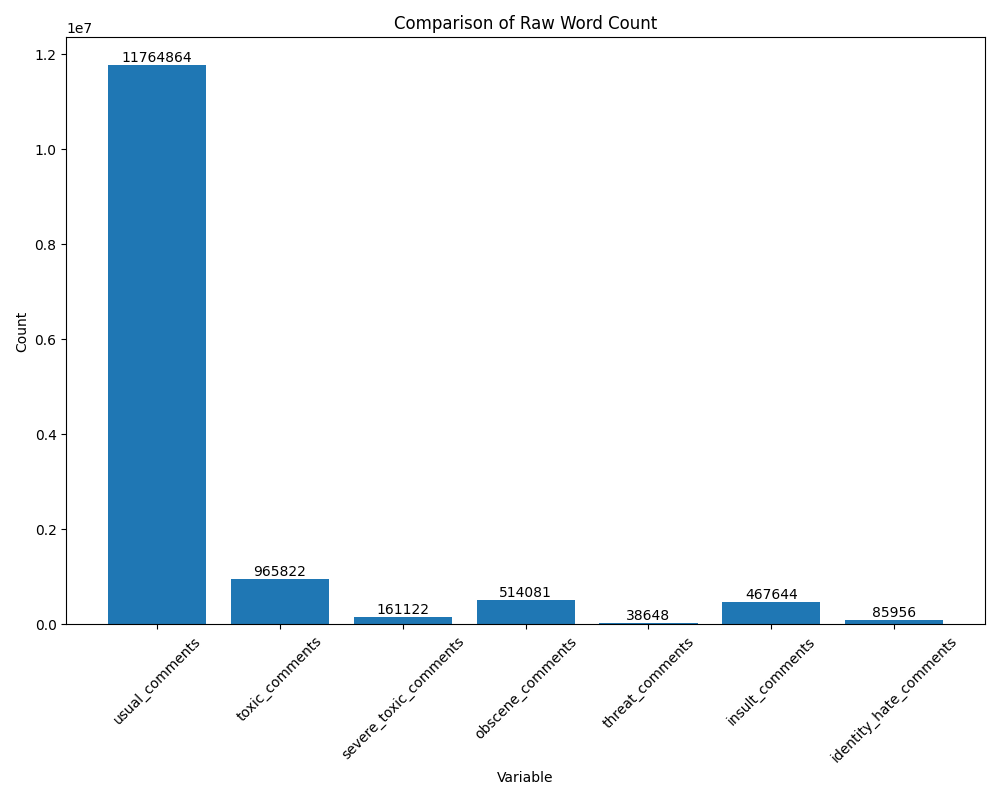
\includegraphics[width=0.8\textwidth]{stats/raw_word_count.png}
  \caption{تعداد کلمات قبل از تمیز کردن}
  \label{fig:raw_word_count}
\end{figure}

\begin{figure}
  \centering
  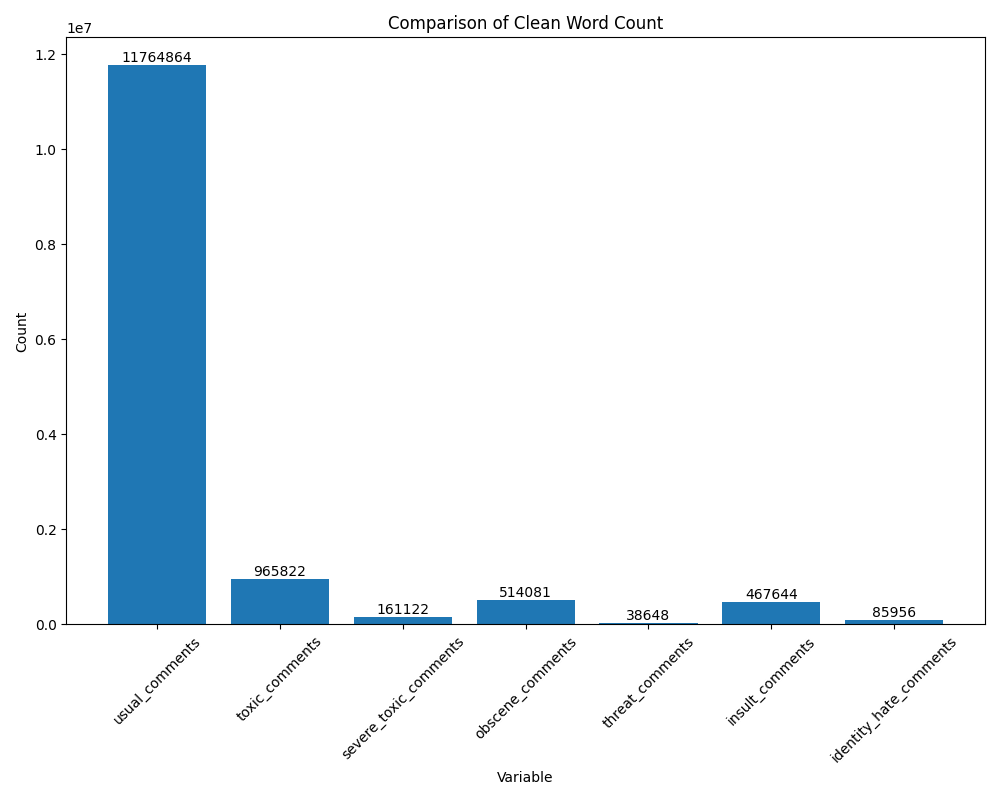
\includegraphics[width=0.8\textwidth]{stats/clean_word_count.png}
  \caption{تعداد کلمات بعد از تمیز کردن}
  \label{fig:clean_word_count}
\end{figure}

\begin{figure}
  \centering
  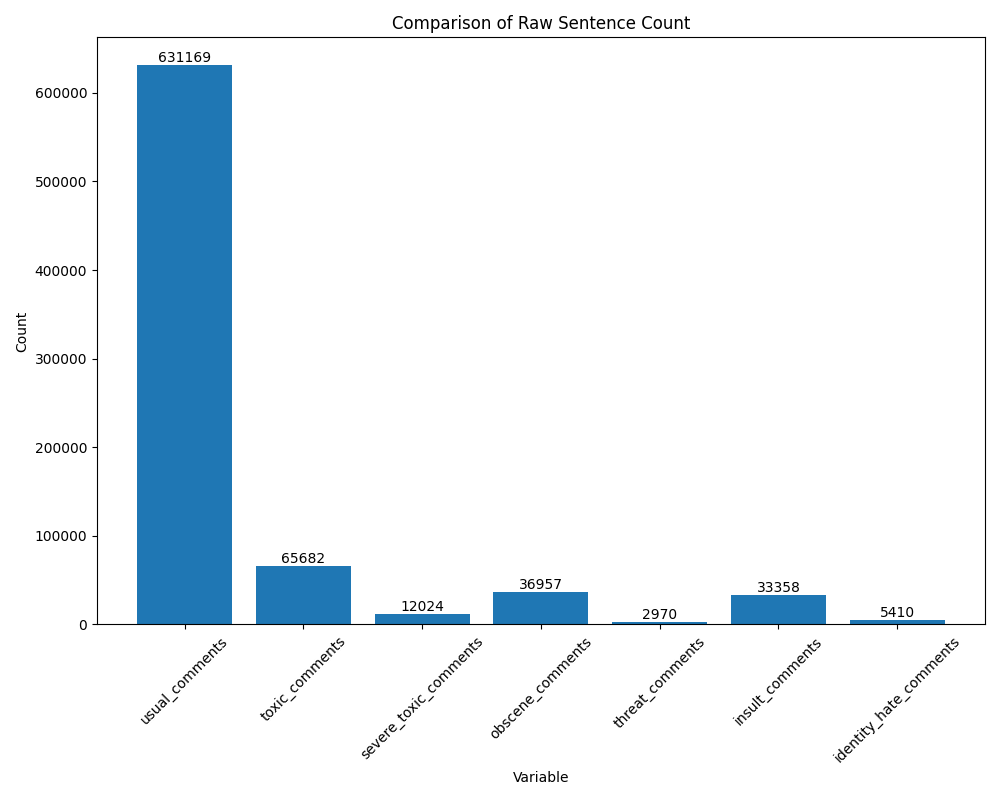
\includegraphics[width=0.8\textwidth]{stats/raw_sentence_count.png}
  \caption{تعداد جملات قبل از تمیز کردن}
  \label{fig:raw_word_count}
\end{figure}

\begin{figure}
  \centering
  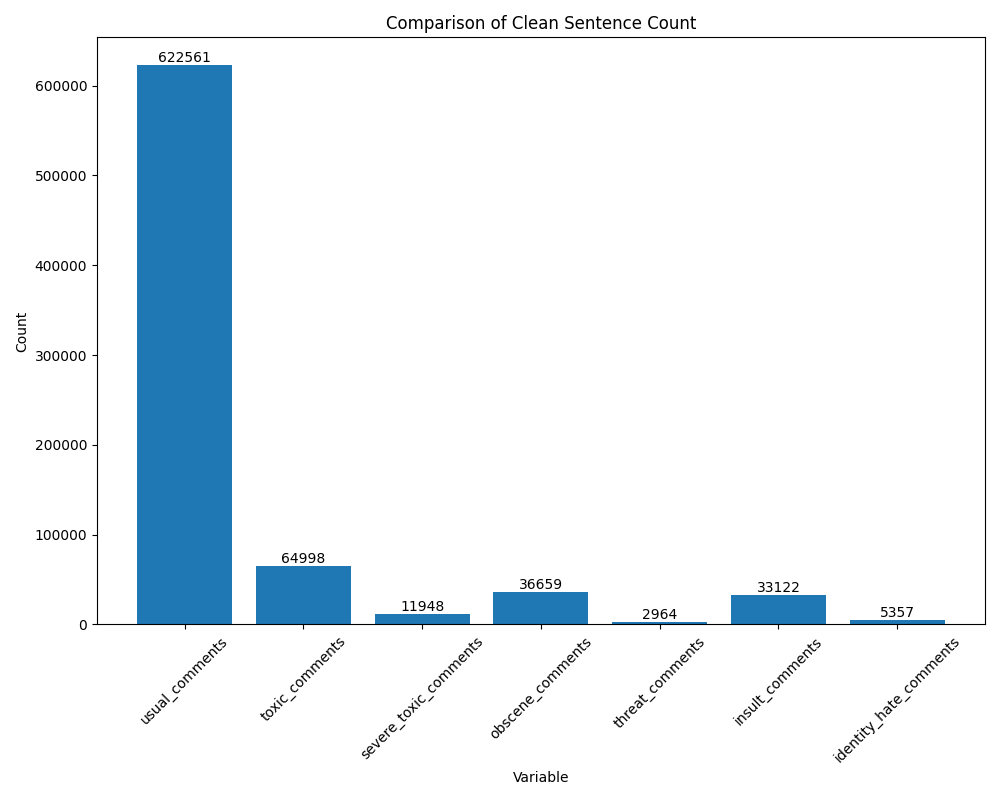
\includegraphics[width=0.8\textwidth]{stats/clean_sentence_count.png}
  \caption{تعداد جملات بعد از تمیز کردن}
  \label{fig:clean_word_count}
\end{figure}

\clearpage

\begin{table}
  \centering
  \begin{subtable}{0.4\textwidth}
    \centering
    \begin{latin}
    \csvautotabular{./stats/clean_word_count.csv}
    \caption{Clean Words Count}
    \label{subfig:file1}
    \end{latin}
  \end{subtable}
  \hspace{2cm}
  \begin{subtable}{0.4\textwidth}
    \centering
    \begin{latin}
    \csvautotabular{stats/raw_word_count.csv}
    \caption{Raw Words Count}
    \label{subfig:file2}
    \end{latin}
  \end{subtable}
  
  \vspace{0.5cm} % Adjust the vertical spacing between the two lines
  
  \begin{subtable}{0.4\textwidth}
    \centering
    \begin{latin}
    \csvautotabular{stats/clean_sentence_count.csv}
    \caption{Clean Sentences Count}
    \label{subfig:file3}
    \end{latin}
  \end{subtable}
  \hfill
  \begin{subtable}{0.4\textwidth}
    \centering
    \begin{latin}
    \csvautotabular{stats/raw_sentence_count.csv}
    \caption{Raw Sentences Count}
    \label{subfig:file4}
    \end{latin}
  \end{subtable}
  
  \caption{جداول تعداد}
  \label{fig:csv_files}
\end{table}

\subsection{بررسی تعداد داده‌های مشترک و غیر مشترک} 
\par
نمودارهای این بخش، به صورت زیر هستند.\\

\begin{figure}
  \centering
  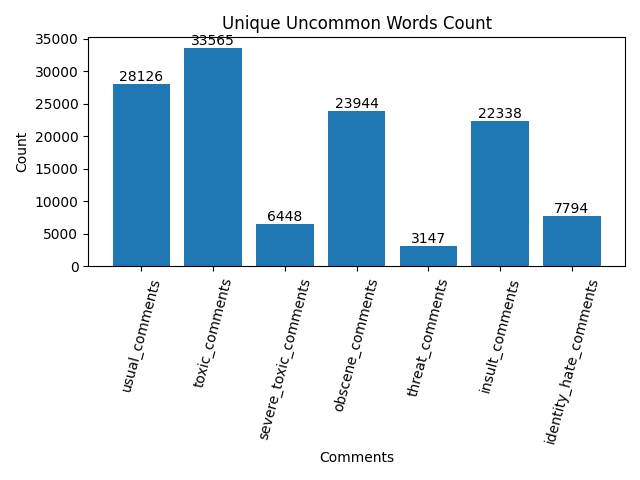
\includegraphics[width=0.8\textwidth]{stats/unique_common_words_total.png}
  \caption{تعداد کلمات مشترک هر دسته}
  \label{fig:unique_common_words_total}
\end{figure}

\begin{figure}
  \centering
  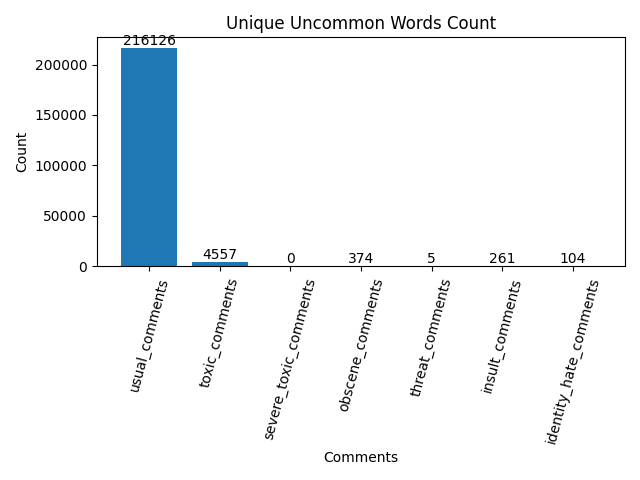
\includegraphics[width=0.8\textwidth]{stats/unique_uncommon_words_count.png}
  \caption{تعداد کلمات غیر مشترک هر دسته}
  \label{fig:unique_uncommon_words_count}
\end{figure}

\clearpage

\begin{table}
  \centering
  \begin{subtable}{0.4\textwidth}
    \centering
    \begin{latin}
    \csvautotabular{stats/unique_common_words_total.csv}
    \end{latin}
    \caption{تعداد کلمات مشترک در هر دسته}
    \label{subfig:unique_common_words_total}
  \end{subtable}
  \hfill
  \begin{subtable}{0.4\textwidth}
    \centering
    \begin{latin}
    \csvautotabular{stats/unique_uncommon_words_count.csv}
    \end{latin}
    \caption{تعداد کلمات غیر مشترک هر دسته}
    \label{subfig:file2}
  \end{subtable}
  
  \caption{جداول کلمات مشترک و غیر مشترک}
  \label{fig:csv_files}
\end{table}

\subsection{بررسی کلمات غیر مشترک هر کلاس} 
\par
در نمودارها و تصاویر زیر، کلمات غیر مشترک پرتکرار هر کلاس آورده شده است.
لازم به ذکر است کلاس \lr{severe toxic} به علت اینکه درجه‌ی سختی بیشتری نسبت به سایر کلاس‌ها داشت، کلمه‌ی مستقلی که در سایر کلاس‌ها نیامده باشد را نداشت.

\begin{figure}[htbp]
  \centering
  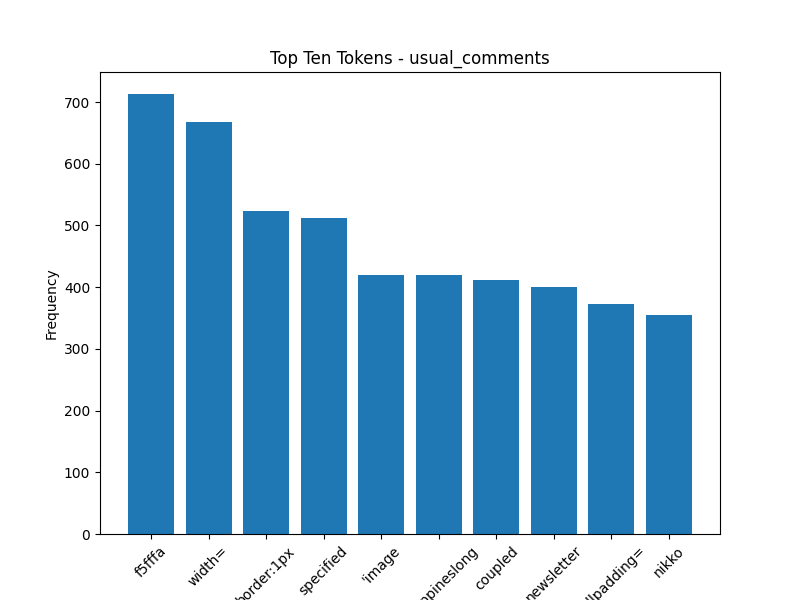
\includegraphics[width=0.8\textwidth]{stats/top_ten_tokens_usual_comments.png}
  \caption{۱۰ کلمه غیر مشترک برتر جملات \lr{usual}}
  \label{fig:unique_common_words_total}
\end{figure}

\begin{figure}
  \centering
  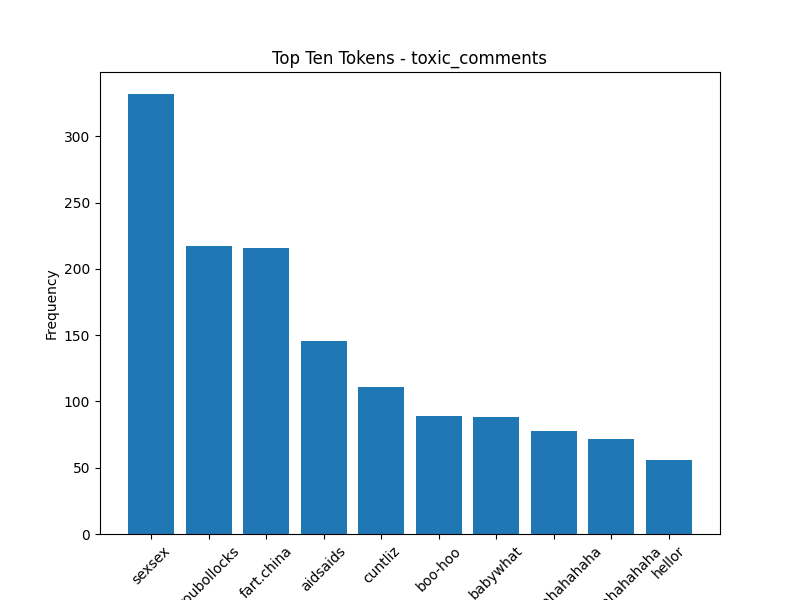
\includegraphics[width=0.8\textwidth]{stats/top_ten_tokens_toxic_comments.png}
  \caption{۱۰ کلمه غیر مشترک برتر جملات \lr{toxic}}
  \label{fig:unique_uncommon_words_count}
\end{figure}

\begin{figure}
  \centering
  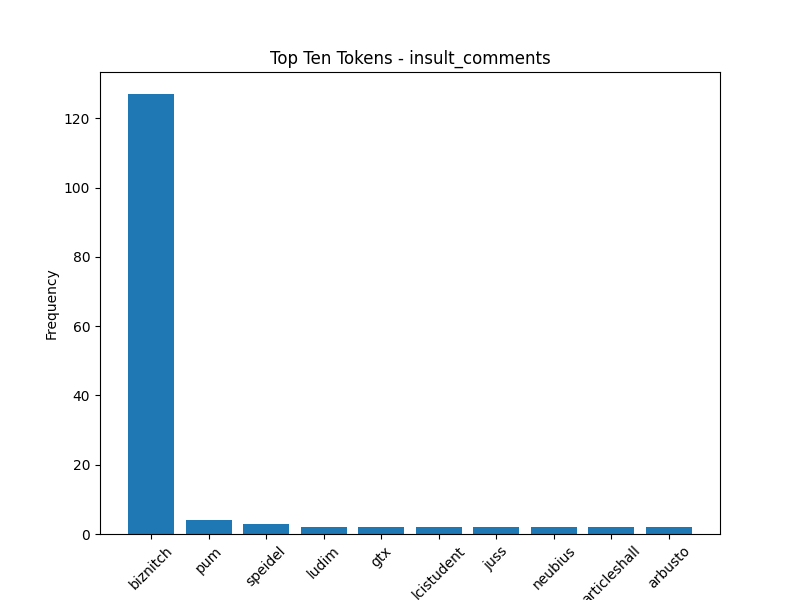
\includegraphics[width=0.8\textwidth]{stats/top_ten_tokens_insult_comments.png}
  \caption{۱۰ کلمه غیر مشترک برتر جملات \lr{insult}}
  \label{fig:unique_common_words_total}
\end{figure}

\begin{figure}
  \centering
  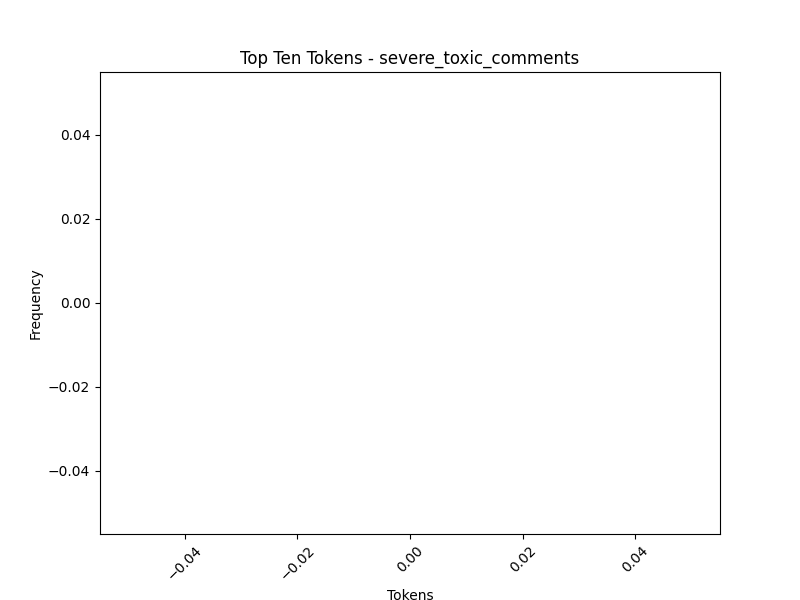
\includegraphics[width=0.8\textwidth]{stats/top_ten_tokens_severe_toxic_comments.png}
  \caption{۱۰ کلمه غیر مشترک برتر جملات \lr{severe toxic}}
  \label{fig:unique_uncommon_words_count}
\end{figure}

\begin{figure}
  \centering
  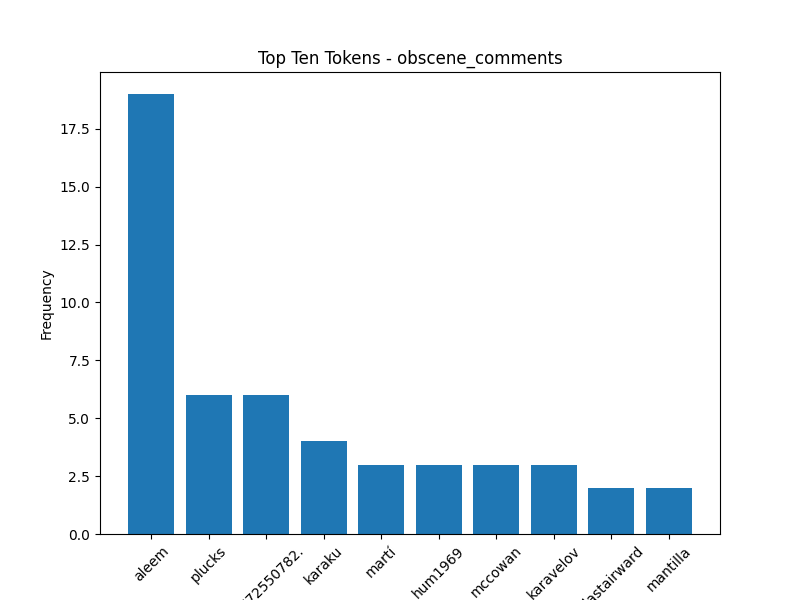
\includegraphics[width=0.8\textwidth]{stats/top_ten_tokens_obscene_comments.png}
  \caption{۱۰ کلمه غیر مشترک برتر جملات \lr{obscene}}
  \label{fig:unique_common_words_total}
\end{figure}

\begin{figure}
  \centering
  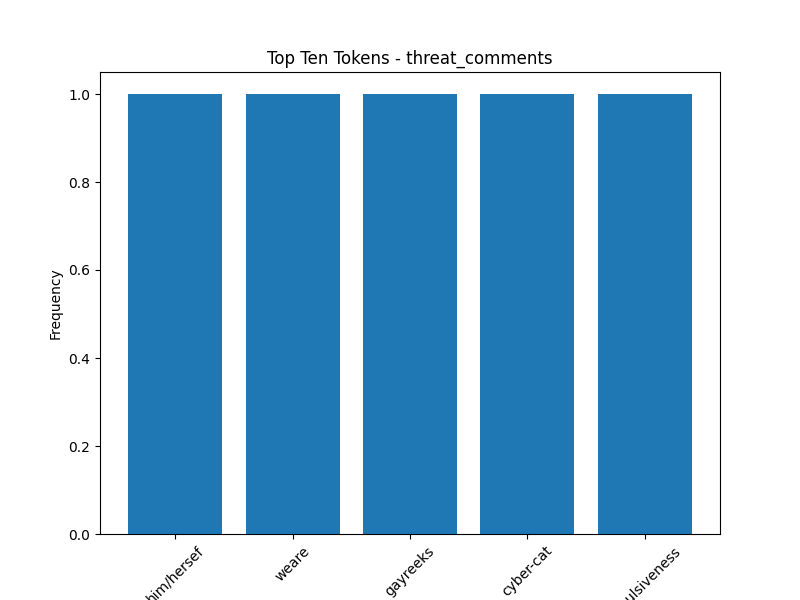
\includegraphics[width=0.8\textwidth]{stats/top_ten_tokens_threat_comments.png}
  \caption{۱۰ کلمه غیر مشترک برتر جملات \lr{threat}}
  \label{fig:unique_uncommon_words_count}
\end{figure}

\begin{figure}
  \centering
  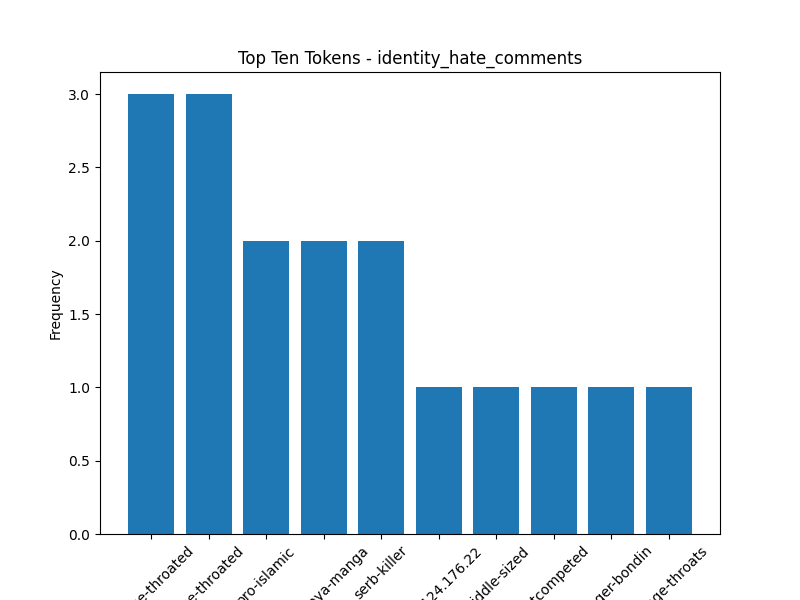
\includegraphics[width=0.8\textwidth]{stats/top_ten_tokens_identity_hate_comments.png}
  \caption{۱۰ کلمه غیر مشترک برتر جملات \lr{identity hate}}
  \label{fig:unique_uncommon_words_count}
\end{figure}

\clearpage

\begin{table}
  \centering
  \begin{subtable}{0.4\textwidth}
    \centering
    \begin{latin}
    \csvautotabular{stats/top_ten_tokens_usual_comments.csv}
    \end{latin}
    \caption{۱۰ کلمه غیر مشترک برتر جملات \lr{usual}}
    \label{subfig:unique_common_words_total}
  \end{subtable}
  \hfill
  \begin{subtable}{0.4\textwidth}
    \centering
    \begin{latin}
    \csvautotabular{stats/top_ten_tokens_toxic_comments.csv}
    \end{latin}
    \caption{۱۰ کلمه غیر مشترک برتر جملات \lr{toxic}}
    \label{subfig:file2}
  \end{subtable}

  \begin{subtable}{0.4\textwidth}
    \centering
    \begin{latin}
        \csvautotabular{stats/top_ten_tokens_insult_comments.csv}
    \end{latin}
    \caption{۱۰ کلمه غیر مشترک برتر جملات \lr{insult}}
    \label{subfig:unique_common_words_total}
  \end{subtable}
  \hfill
  \begin{subtable}{0.4\textwidth}
    \centering
    \begin{latin}
    \csvautotabular{stats/top_ten_tokens_severe_toxic_comments.csv}
    \end{latin}
    \caption{۱۰ کلمه غیر مشترک برتر جملات \lr{severe toxic}}
    \label{subfig:file2}
  \end{subtable}

  \begin{subtable}{0.4\textwidth}
    \centering
    \begin{latin}
    \csvautotabular{stats/top_ten_tokens_obscene_comments.csv}
    \end{latin}
    \caption{۱۰ کلمه غیر مشترک برتر جملات \lr{obscene}}
    \label{subfig:unique_common_words_total}
  \end{subtable}
  \hfill
  \begin{subtable}{0.4\textwidth}
    \centering
    \begin{latin}
    \csvautotabular{stats/top_ten_tokens_identity_hate_comments.csv}
    \end{latin}
    \caption{۱۰ کلمه غیر مشترک برتر جملات \lr{identity hate}}
    \label{subfig:unique_common_words_total}
  \end{subtable}

  \begin{subtable}{0.4\textwidth}
    \centering
    \begin{latin}
    \csvautotabular{stats/top_ten_tokens_threat_comments.csv}
    \end{latin}
    \caption{۱۰ کلمه غیر مشترک برتر جملات \lr{threat}}
    \label{subfig:unique_common_words_total}
  \end{subtable}

  \label{fig:csv_files}
\end{table}

\clearpage

\subsection{امتیازات کلمات هر دسته بر حسب RNE}
در این قسمت از گزارش، برای هر دسته، ۱۰ کلمه با بیشترین امتیاز طبق معیار توضیح داده شده در داکیومنت پروژه یعنی RNE آورده شده است.

\begin{figure}[htbp]
  \centering
  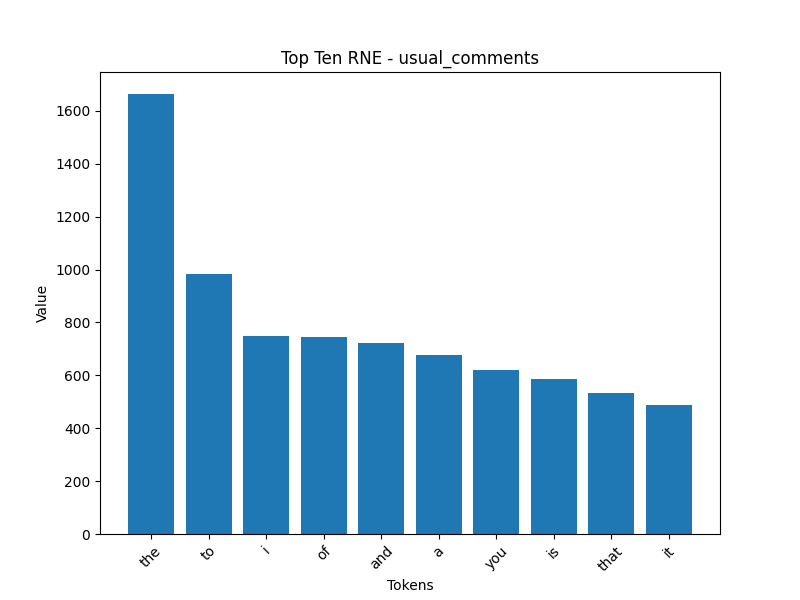
\includegraphics[width=0.8\textwidth]{stats/top_ten_RNE_usual_comments.png}
  \caption{۱۰ کلمه برتر جملات usual}
  \label{fig:unique_common_words_total}
\end{figure}

\begin{figure}[htbp]
  \centering
  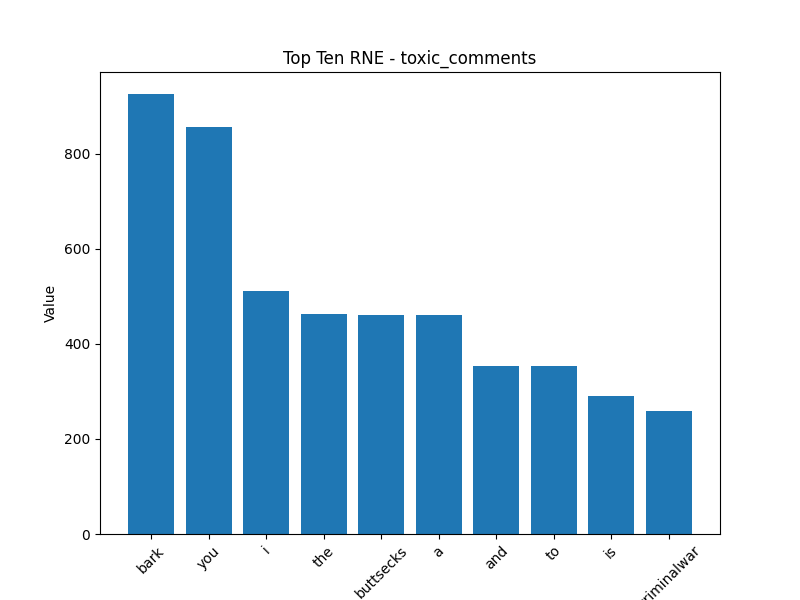
\includegraphics[width=0.8\textwidth, height=5.25cm]{stats/top_ten_RNE_toxic_comments.png}
  \caption{۱۰ کلمه برتر جملات \lr{toxic}}
  \label{fig:unique_uncommon_words_count}
\end{figure}

\begin{figure}
  \centering
  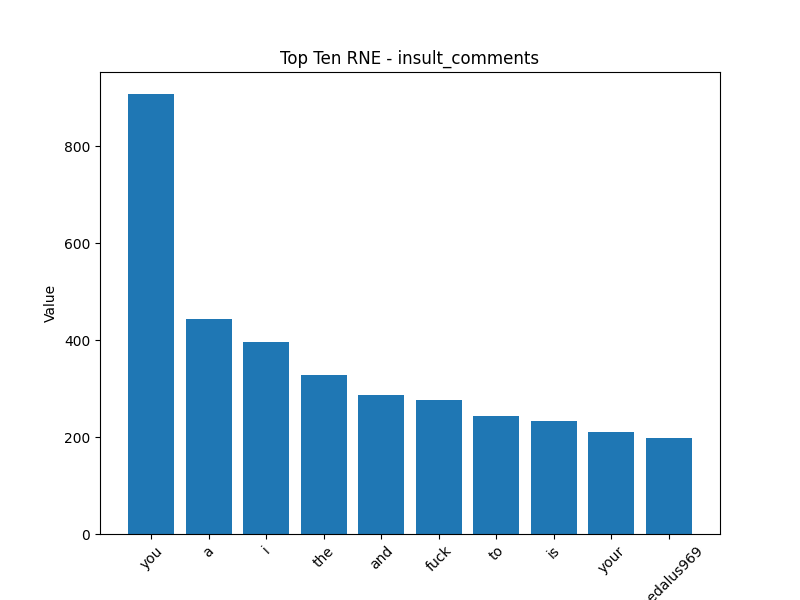
\includegraphics[width=0.8\textwidth]{stats/top_ten_RNE_insult_comments.png}
  \caption{۱۰ کلمه برتر جملات \lr{insult}}
  \label{fig:unique_common_words_total}
\end{figure}

\begin{figure}
  \centering
  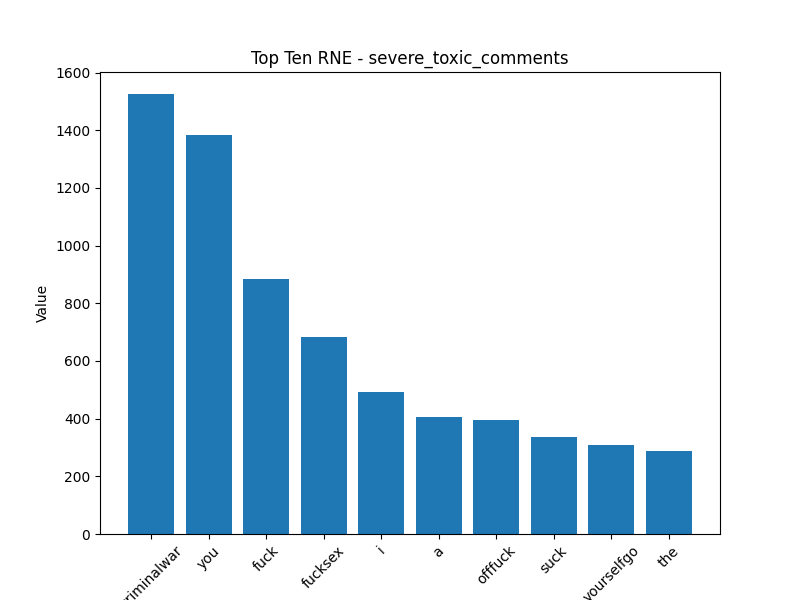
\includegraphics[width=0.8\textwidth]{stats/top_ten_RNE_severe_toxic_comments.png}
  \caption{۱۰ کلمه برتر جملات \lr{severe toxic}}
  \label{fig:unique_uncommon_words_count}
\end{figure}

\begin{figure}
  \centering
  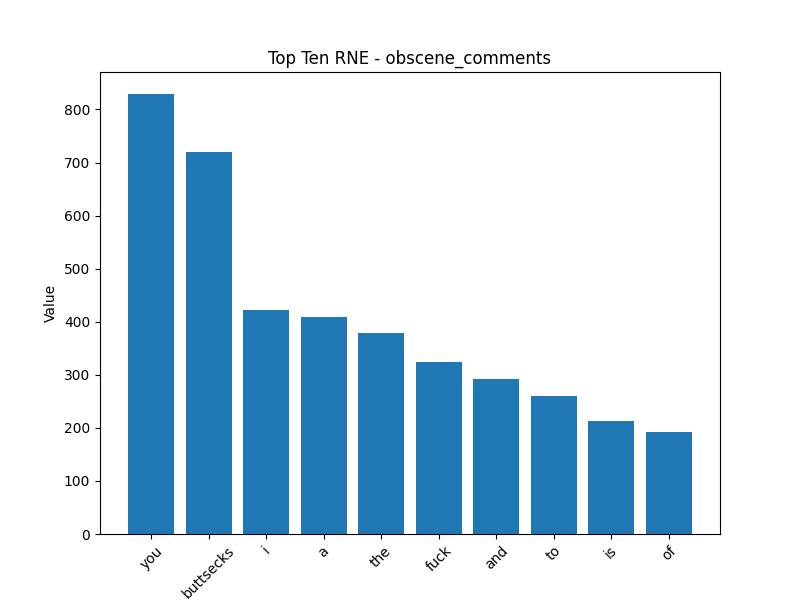
\includegraphics[width=0.8\textwidth]{stats/top_ten_RNE_obscene_comments.png}
  \caption{۱۰ کلمه برتر جملات \lr{obscene}}
  \label{fig:unique_common_words_total}
\end{figure}

\begin{figure}
  \centering
  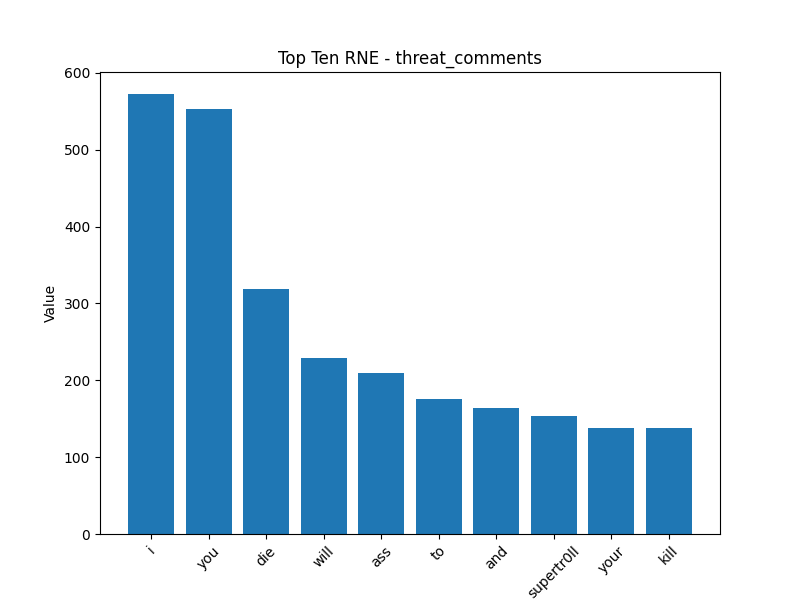
\includegraphics[width=0.8\textwidth]{stats/top_ten_RNE_threat_comments.png}
  \caption{۱۰ کلمه برتر جملات \lr{threat}}
  \label{fig:unique_uncommon_words_count}
\end{figure}

\begin{figure}
  \centering
  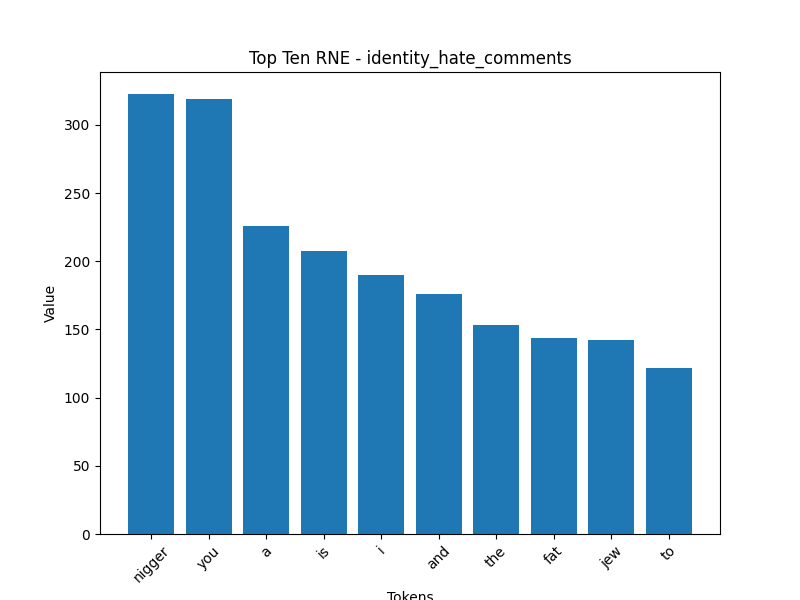
\includegraphics[width=0.8\textwidth]{stats/top_ten_RNE_identity_hate_comments.png}
  \caption{۱۰ کلمه برتر جملات \lr{identity hate}}
  \label{fig:unique_uncommon_words_count}
\end{figure}

\clearpage

\begin{table}[htbp]
  \centering
  \begin{subtable}{0.4\textwidth}
    \centering
    \begin{latin}
    \csvautotabular{stats/top_ten_RNE_usual_comments.csv}
    \end{latin}
    \caption{۱۰ کلمه برتر جملات \lr{usual}}
    \label{subfig:unique_common_words_total}
  \end{subtable}
  \hfill
  \begin{subtable}{0.4\textwidth}
    \centering
    \begin{latin}
    \csvautotabular{stats/top_ten_RNE_toxic_comments.csv}
    \end{latin}
    \caption{۱۰ کلمه برتر جملات \lr{toxic}}
    \label{subfig:file2}
  \end{subtable}

  \begin{subtable}{0.4\textwidth}
    \centering
    \begin{latin}
    \csvautotabular{stats/top_ten_RNE_insult_comments.csv}
    \end{latin}
    \caption{۱۰ کلمه برتر جملات \lr{insult}}
    \label{subfig:unique_common_words_total}
  \end{subtable}
  \hfill
  \begin{subtable}{0.4\textwidth}
    \centering
    \begin{latin}
    \csvautotabular{stats/top_ten_RNE_severe_toxic_comments.csv}
    \end{latin}
    \caption{۱۰ کلمه برتر جملات \lr{severe toxic}}
    \label{subfig:file2}
  \end{subtable}

  \begin{subtable}{0.4\textwidth}
    \centering
    \begin{latin}
    \csvautotabular{stats/top_ten_RNE_obscene_comments.csv}
    \end{latin}
    \caption{۱۰ کلمه برتر جملات \lr{obscene}}
    \label{subfig:unique_common_words_total}
  \end{subtable}
  \hfill
  \begin{subtable}{0.4\textwidth}
    \centering
    \begin{latin}
    \csvautotabular{stats/top_ten_RNE_identity_hate_comments.csv}
    \end{latin}
    \caption{۱۰ کلمه برتر جملات \lr{identity hate}}
    \label{subfig:unique_common_words_total}
  \end{subtable}
  
  \label{fig:csv_files}
\end{table}

\clearpage

\afterpage{
  \begin{table}
    \ContinuedFloat
    \centering
    \begin{subtable}{0.4\textwidth}
      \centering
      \begin{latin}
      \csvautotabular{stats/top_ten_RNE_threat_comments.csv}
      \end{latin}
      \caption{۱۰ کلمه برتر جملات threat}
      \label{subfig:unique_common_words_total}
    \end{subtable}
    \caption*{جدوال مربوط به امتیازات \lr{RNE} در هر دسته}
    \label{fig:last_csv_file}
  \end{table}
}

\clearpage

\subsection{امتیازات کلمات هر دسته بر حسب \lr{TF-IDF}} 
\par
در این قسمت از گزارش، برای هر دسته، ۱۰ کلمه با بیشترین امتیاز طبق معیار توضیح داده شده در داکیومنت پروژه یعنی \lr{TF-IDF} آورده شده است. 


\begin{figure}
  \centering
  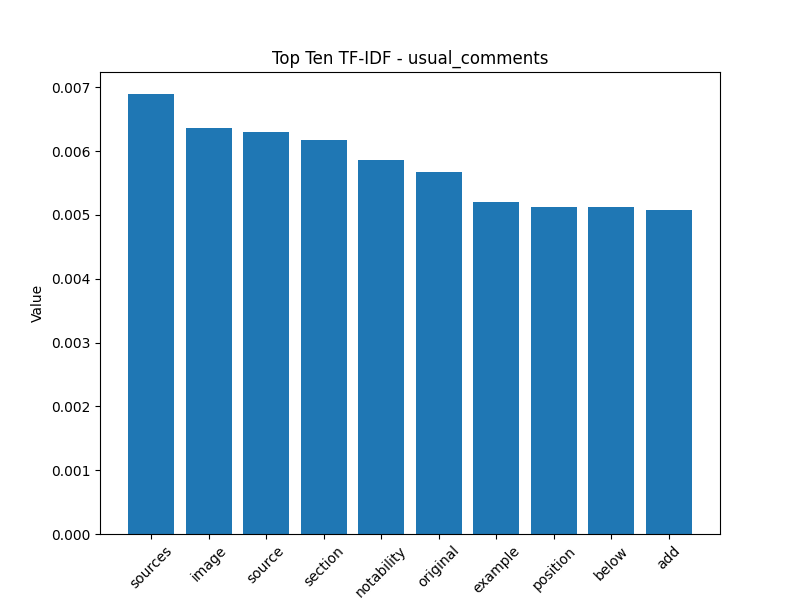
\includegraphics[width=0.8\textwidth]{stats/top_ten_TF-IDF_usual_comments.png}
  \caption{۱۰ کلمه برتر جملات \lr{usual}}
  \label{fig:unique_common_words_total}
\end{figure}

\begin{figure}
  \centering
  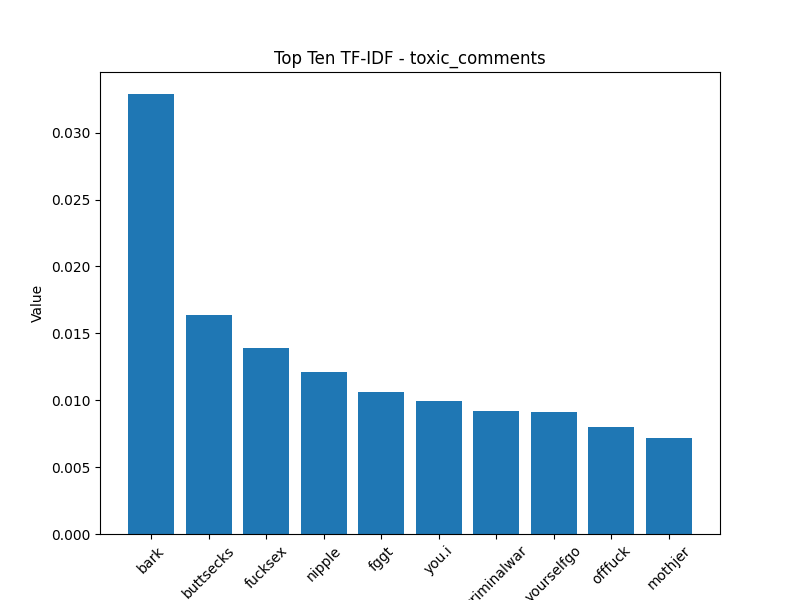
\includegraphics[width=0.8\textwidth]{stats/top_ten_TF-IDF_toxic_comments.png}
  \caption{۱۰ کلمه برتر جملات \lr{toxic}}
  \label{fig:unique_uncommon_words_count}
\end{figure}

\begin{figure}
  \centering
  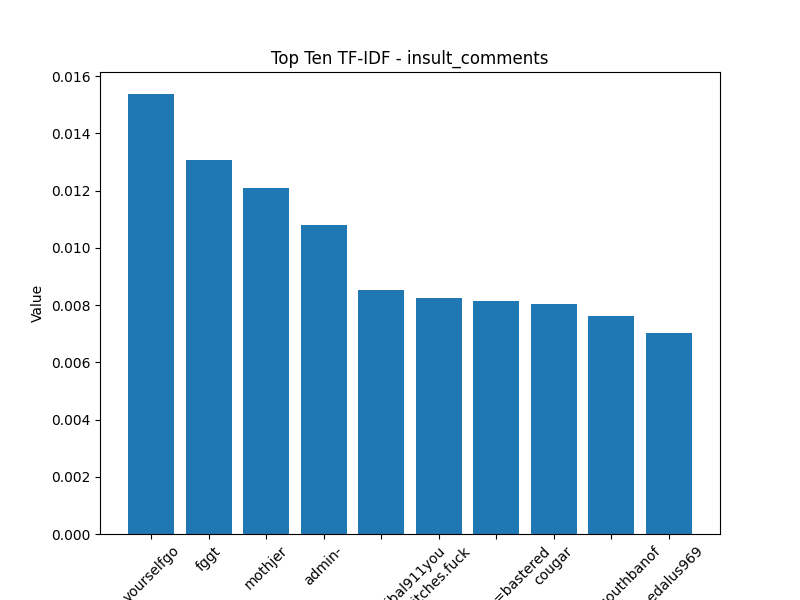
\includegraphics[width=0.8\textwidth]{stats/top_ten_TF-IDF_insult_comments.png}
  \caption{۱۰ کلمه برتر جملات \lr{insult}}
  \label{fig:unique_common_words_total}
\end{figure}

\begin{figure}
  \centering
  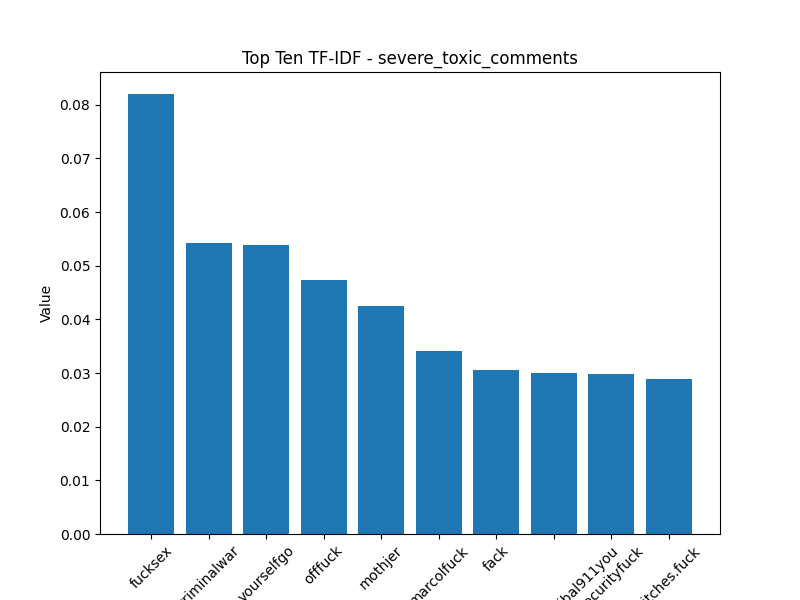
\includegraphics[width=0.8\textwidth]{stats/top_ten_TF-IDF_severe_toxic_comments.png}
  \caption{۱۰ کلمه برتر جملات \lr{severe toxic}}
  \label{fig:unique_uncommon_words_count}
\end{figure}

\begin{figure}
  \centering
  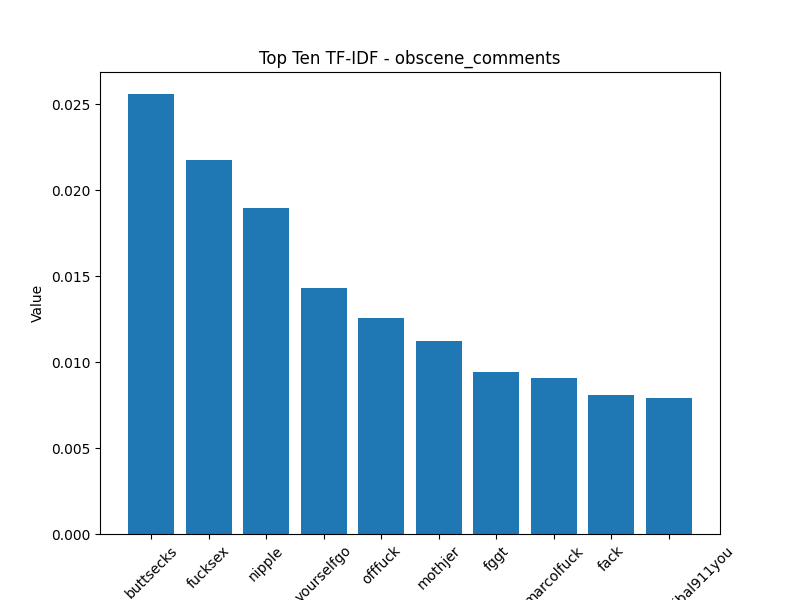
\includegraphics[width=0.8\textwidth]{stats/top_ten_TF-IDF_obscene_comments.png}
  \caption{۱۰ کلمه برتر جملات \lr{obscene}}
  \label{fig:unique_common_words_total}
\end{figure}

\begin{figure}
  \centering
  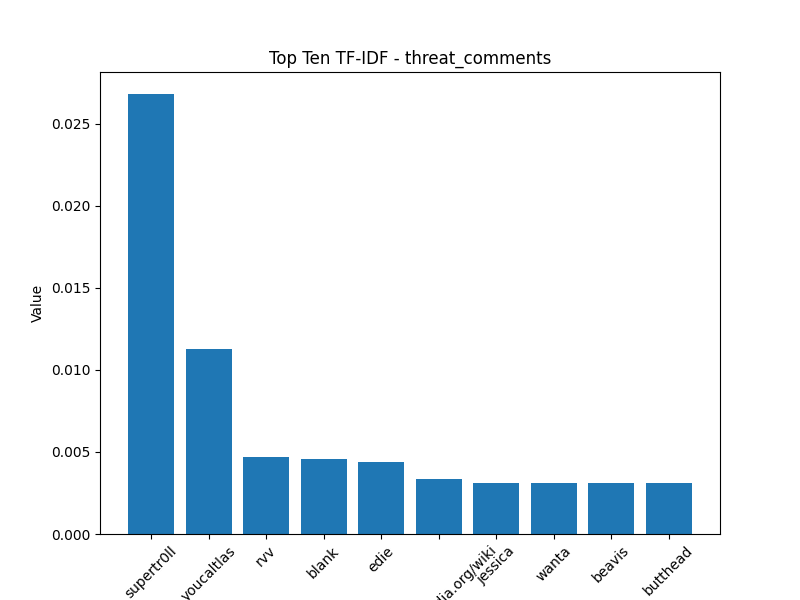
\includegraphics[width=0.8\textwidth]{stats/top_ten_TF-IDF_threat_comments.png}
  \caption{۱۰ کلمه برتر جملات \lr{threat}}
  \label{fig:unique_uncommon_words_count}
\end{figure}

\begin{figure}
  \centering
  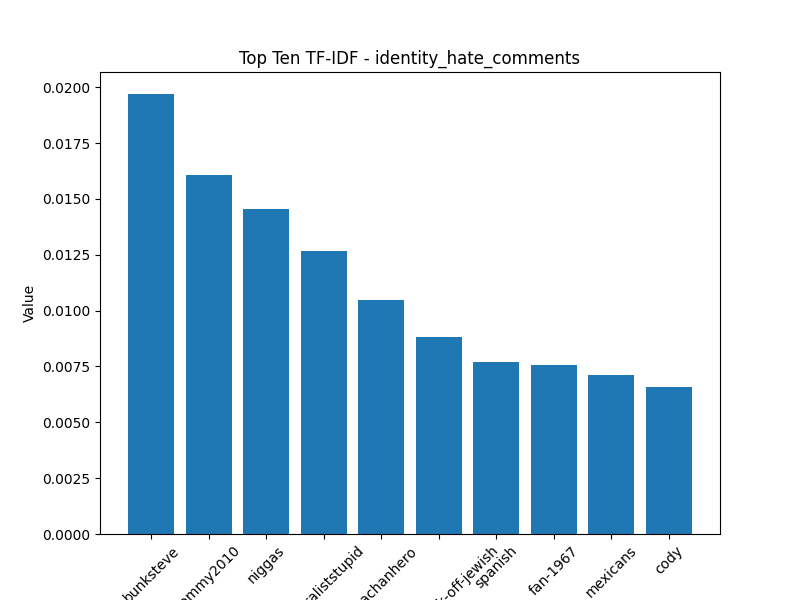
\includegraphics[width=0.8\textwidth]{stats/top_ten_TF-IDF_identity_hate_comments.png}
  \caption{۱۰ کلمه برتر جملات \lr{identity hate}}
  \label{fig:unique_uncommon_words_count}
\end{figure}

\clearpage

\begin{table}
  \centering
  \begin{subtable}{0.4\textwidth}
    \centering
    \begin{latin}
    \csvautotabular{stats/top_ten_TF-IDF_usual_comments.csv}
    \end{latin}
    \caption{۱۰ کلمه برتر جملات \lr{usual}}
    \label{subfig:unique_common_words_total}
  \end{subtable}
  \hfill
  \begin{subtable}{0.4\textwidth}
    \centering
    \begin{latin}
    \csvautotabular{stats/top_ten_TF-IDF_toxic_comments.csv}
    \end{latin}
    \caption{۱۰ کلمه برتر جملات \lr{toxic}}
    \label{subfig:file2}
  \end{subtable}

  \begin{subtable}{0.4\textwidth}
    \centering
    \begin{latin}
    \csvautotabular{stats/top_ten_TF-IDF_insult_comments.csv}
    \end{latin}
    \caption{۱۰ کلمه برتر جملات \lr{insult}}
    \label{subfig:unique_common_words_total}
  \end{subtable}
  \hfill
  \begin{subtable}{0.4\textwidth}
    \centering
    \begin{latin}
    \csvautotabular{stats/top_ten_TF-IDF_severe_toxic_comments.csv}
    \end{latin}
    \caption{۱۰ کلمه برتر جملات \lr{severe toxic}}
    \label{subfig:file2}
  \end{subtable}

  \begin{subtable}{0.4\textwidth}
    \centering
    \begin{latin}
    \csvautotabular{stats/top_ten_TF-IDF_obscene_comments.csv}
    \end{latin}
    \caption{۱۰ کلمه برتر جملات \lr{obscene}}
    \label{subfig:unique_common_words_total}
  \end{subtable}
  \hfill
  \begin{subtable}{0.4\textwidth}
    \centering
    \begin{latin}
    \csvautotabular{stats/top_ten_TF-IDF_identity_hate_comments.csv}
    \end{latin}
    \caption{۱۰ کلمه برتر جملات \lr{identity hate}}
    \label{subfig:unique_common_words_total}
  \end{subtable}
  
  \label{fig:csv_files}
\end{table}

\clearpage

\afterpage{
  \begin{table}
    \ContinuedFloat
    \centering
    \begin{subtable}{0.4\textwidth}
      \centering
      \begin{latin}
      \csvautotabular{stats/top_ten_TF-IDF_threat_comments.csv}
      \end{latin}
      \caption{۱۰ کلمه برتر جملات \lr{threat}}
      \label{subfig:unique_common_words_total}
    \end{subtable}
    \caption*{جدوال مربوط به امتیازات \lr{TF-IDF} در هر دسته}
    \label{fig:last_csv_file}
  \end{table}
}

\clearpage

\subsection{هیستوگرام کلمات پر تکرار} 

\begin{figure}[htbp]
  \centering
  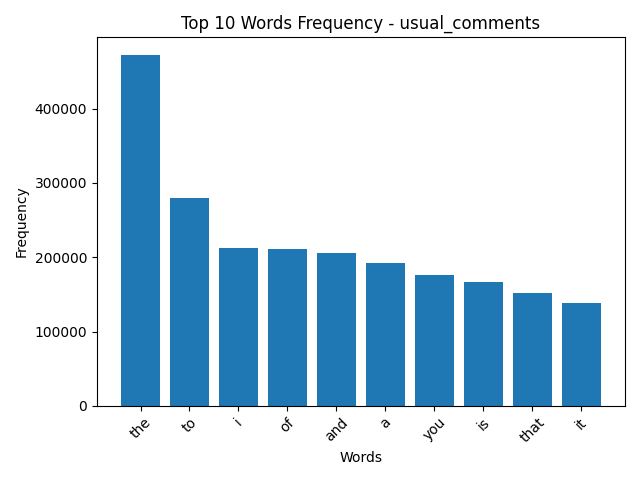
\includegraphics[width=0.8\textwidth]{stats/top_ten_histogram_usual_comments.png}
  \caption{۱۰ کلمه برتر جملات \lr{usual}}
  \label{fig:unique_common_words_total}
\end{figure}

\begin{figure}
  \centering
  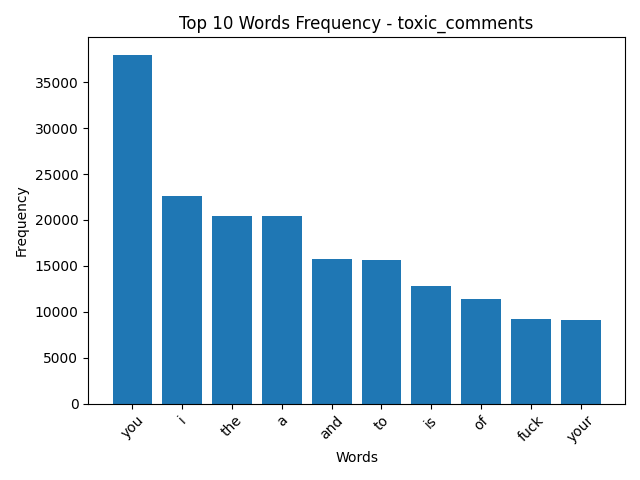
\includegraphics[width=0.8\textwidth]{stats/top_ten_histogram_toxic_comments.png}
  \caption{۱۰ کلمه برتر جملات \lr{toxic}}
  \label{fig:unique_uncommon_words_count}
\end{figure}

\begin{figure}
  \centering
  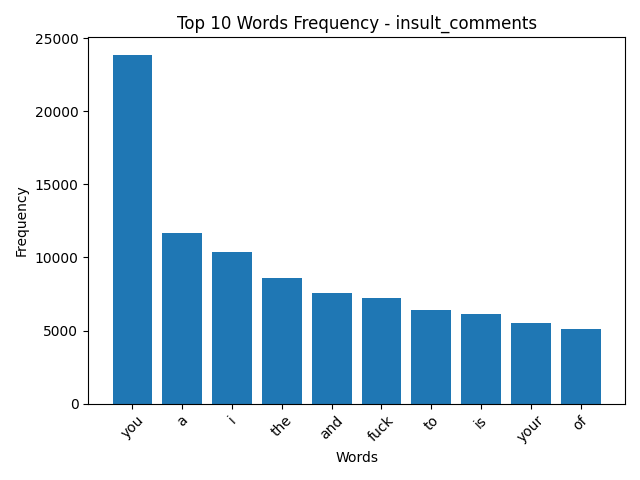
\includegraphics[width=0.8\textwidth]{stats/top_ten_histogram_insult_comments.png}
  \caption{۱۰ کلمه برتر جملات \lr{insult}}
  \label{fig:unique_common_words_total}
\end{figure}

\begin{figure}
  \centering
  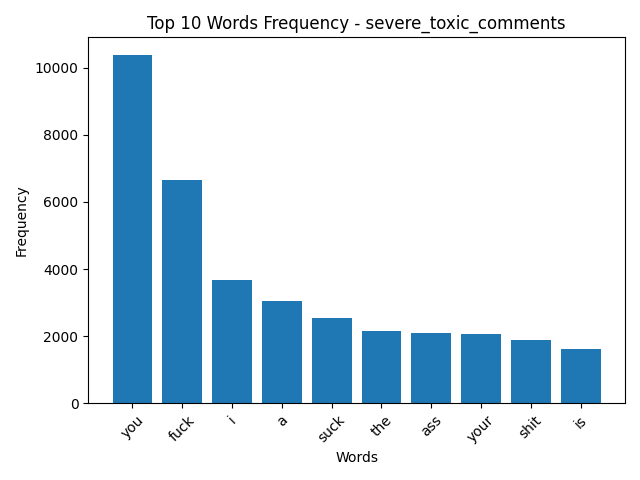
\includegraphics[width=0.8\textwidth]{stats/top_ten_histogram_severe_toxic_comments.png}
  \caption{۱۰ کلمه برتر جملات \lr{severe toxic}}
  \label{fig:unique_uncommon_words_count}
\end{figure}

\begin{figure}
  \centering
  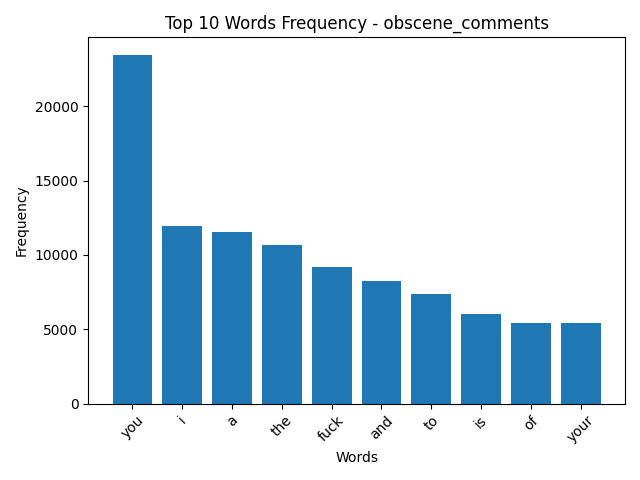
\includegraphics[width=0.8\textwidth]{stats/top_ten_histogram_obscene_comments.png}
  \caption{۱۰ کلمه برتر جملات \lr{obscene}}
  \label{fig:unique_common_words_total}
\end{figure}

\begin{figure}
  \centering
  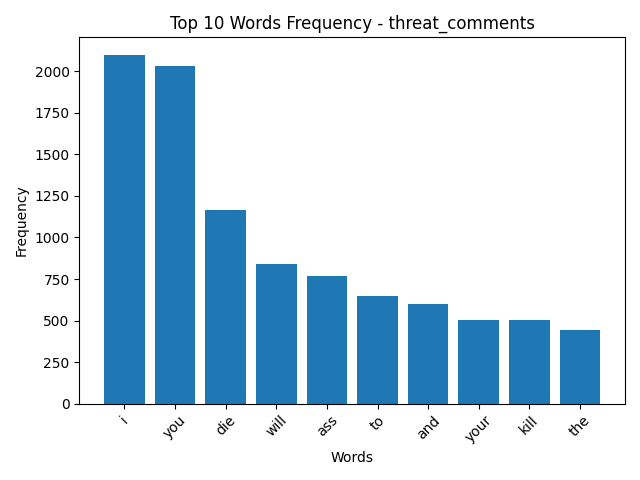
\includegraphics[width=0.8\textwidth]{stats/top_ten_histogram_threat_comments.png}
  \caption{۱۰ کلمه برتر جملات \lr{threat}}
  \label{fig:unique_uncommon_words_count}
\end{figure}

\begin{figure}
  \centering
  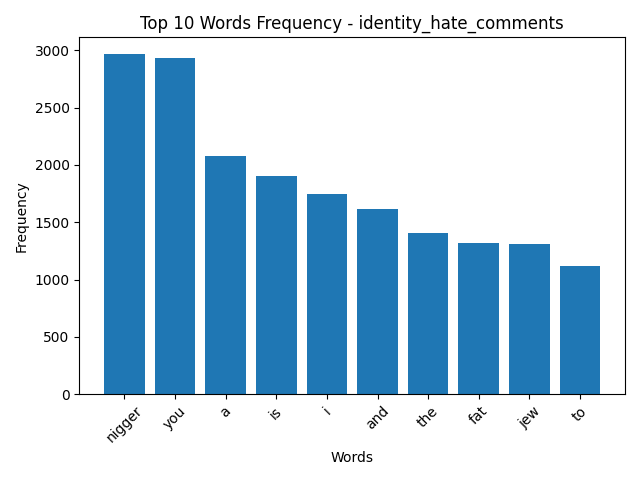
\includegraphics[width=0.8\textwidth]{stats/top_ten_histogram_identity_hate_comments.png}
  \caption{۱۰ کلمه برتر جملات \lr{identity hate}}
  \label{fig:unique_uncommon_words_count}
\end{figure}

\clearpage

\begin{table}
  \centering
  \begin{subtable}{0.4\textwidth}
    \centering
    \begin{latin}
    \csvautotabular{stats/top_ten_histogram_usual_comments.csv}
    \end{latin}
    \caption{۱۰ کلمه برتر جملات \lr{usual}}
    \label{subfig:unique_common_words_total}
  \end{subtable}
  \hfill
  \begin{subtable}{0.4\textwidth}
    \centering
    \begin{latin}
    \csvautotabular{stats/top_ten_histogram_toxic_comments.csv}
    \end{latin}
    \caption{۱۰ کلمه برتر جملات \lr{toxic}}
    \label{subfig:file2}
  \end{subtable}

  \begin{subtable}{0.4\textwidth}
    \centering
    \begin{latin}
    \csvautotabular{stats/top_ten_histogram_insult_comments.csv}
    \end{latin}
    \caption{۱۰ کلمه برتر جملات \lr{insult}}
    \label{subfig:unique_common_words_total}
  \end{subtable}
  \hfill
  \begin{subtable}{0.4\textwidth}
    \centering
    \begin{latin}
    \csvautotabular{stats/top_ten_histogram_severe_toxic_comments.csv}
    \end{latin}
    \caption{۱۰ کلمه برتر جملات \lr{severe toxic}}
    \label{subfig:file2}
  \end{subtable}

  \begin{subtable}{0.4\textwidth}
    \centering
    \begin{latin}
    \csvautotabular{stats/top_ten_histogram_obscene_comments.csv}
    \end{latin}
    \caption{۱۰ کلمه برتر جملات \lr{obscene}}
    \label{subfig:unique_common_words_total}
  \end{subtable}
  \hfill
  \begin{subtable}{0.4\textwidth}
    \centering
    \begin{latin}
    \csvautotabular{stats/top_ten_histogram_identity_hate_comments.csv}
    \end{latin}
    \caption{۱۰ کلمه برتر جملات \lr{identity hate}}
    \label{subfig:unique_common_words_total}
  \end{subtable}
  
  \label{fig:csv_files}
\end{table}

\clearpage

\afterpage{
  \begin{table}
    \ContinuedFloat
    \centering
    \begin{subtable}{0.4\textwidth}
      \centering
      \begin{latin}
      \csvautotabular{stats/top_ten_histogram_threat_comments.csv}
      \end{latin}
      \caption{۱۰ کلمه برتر جملات \lr{threat}}
      \label{subfig:unique_common_words_total}
    \end{subtable}
    \caption*{جدوال مربوط به امتیازات \lr{histogram} در هر دسته}
    \label{fig:last_csv_file}
  \end{table}
}

\clearpage

